\documentclass[a4paper,12pt]{article}
\usepackage{hyperref}
\usepackage{times}
\usepackage{comment}
\usepackage{titlesec}
\usepackage[pdftex]{graphicx}

\usepackage{geometry}
\geometry{lmargin=1.5cm,rmargin=1.5cm,height=25cm}
\renewcommand{\thesubsection}{\Roman{subsection}}

\begin{document}
\title{ASPECTS OF A SHIPWRECK -- St. Paul on Malta}
\author{Joanna Lace}
\date{}
\maketitle


\begin{center}
\parbox{5.5truein}{ ``...the word has universal authority, [whereas]
  the image is always individual and specific, one aspect only out of
  the many that we know exist.''\hfill Neil McGregor\footnotemark.  }
\footnotetext{A quotation from Neil McGregor's Introduction to
  G.~Finaldi et al., \textit{The Image of Christ}: catalogue of the
  exhibition \textit{Seeing Salvation}, The National Gallery, London,
  2000, pp.6--7. }
\end{center}

This essay takes up the suggestion of Neil McGregor that in order to
acquire a deeper understanding of a religious subject, we need
`different aspects, different visions'. It would be difficult to find
visions that at first sight differ more fundamentally in their
approach than those of certain artists depicting the arrival of
St.~Paul on the island of Malta: we examine a few in detail,
irrespective of their date or context, in McGregor's fashion.

We begin with a work familiar in Malta itself, an altarpiece by
Stefano Eradi for St.~Paul's Collegiate Church in Rabat. [Fig. 1] 
\begin{figure}[htbp]
\centering
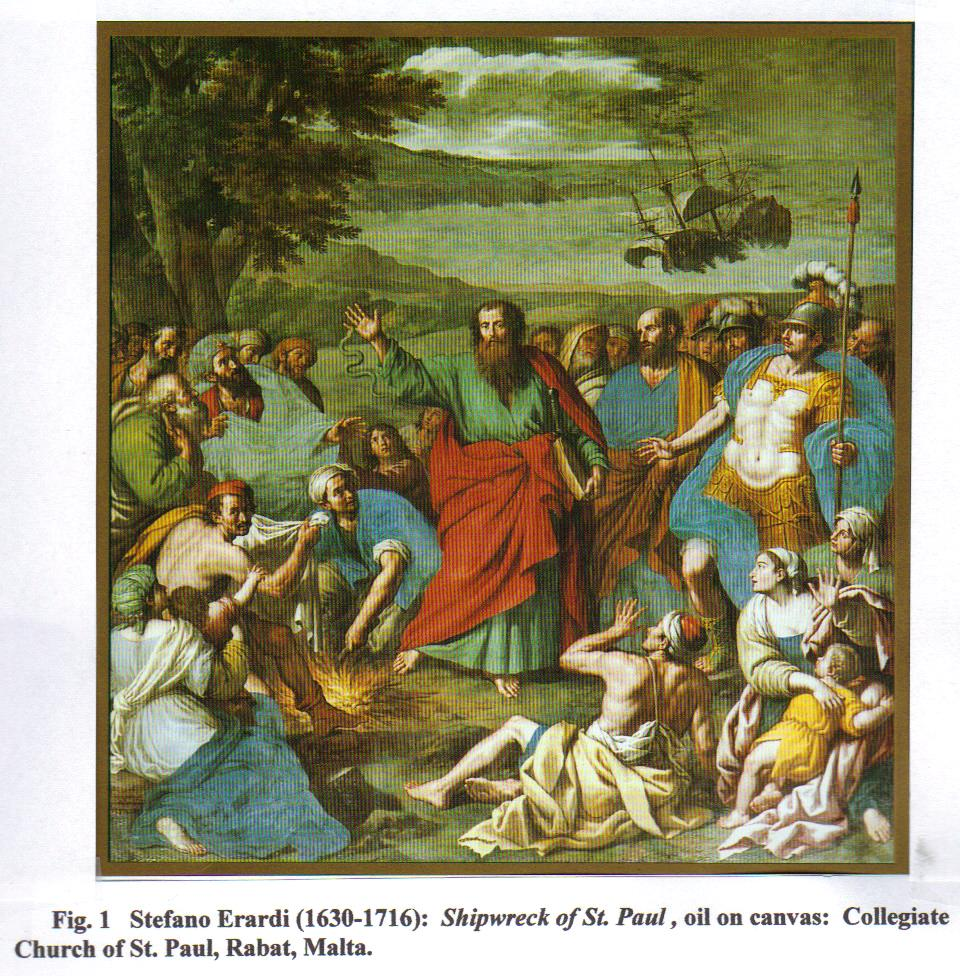
\includegraphics[width=10cm]{fig1.jpg}
%\caption[Fig.~1]{}
\end{figure}
Here
a wrecked ship identifies the scene, but is not relegated, as in other
local versions, to a distant coast shown in the upper section as a
simple mark of recognition for the event.  This artist plans the
entire scene in accordance with the classic `rule of enclosure': to
this effect both ship and coastline are brought nearer to the action,
and placed to the right of the panel so that darker areas of vessel
and leaden sky can be seen as joining the tree on the left side to
form a great arch over the heavens, uniting within an all-encompassing
frame the activity beneath.  And here the `heroic' figure of St.~Paul
dominates a group of other passengers who have reached the shore,
standing with his right arm raised high as he shakes off the snake.
He is placed exactly at centre-stage, for we are watching a
classically centralised drama, the aim of which is the ennoblement of
the figure by means of its centrality and the symmetry of the
surrounding circle of activity.  Eradi's figures are in fact an
interesting mix of the classical and the mannerist, in which the
posture of each figure has been individually conceived: for the main
protagonists there is decorum, solidity, and for minor figures, exempt
from decorum, the freedom to display emotions by facial expression, by
a fanning out of the fingers or similar demonstrative
gesture\footnote{Amongst the crowd, near the left margin, the artist
  Stefano Eradi (l630--1716) has included his self-portrait: he turns
  to the viewer and gestures towards St.~Paul.  The sources of
  St.Paul's idealised head, clothing and pose are identified by Gerald
  Bugeja in `From Eradi to Zahra: the Emilian Connectio', in
  ed. J. Azzopardi, \textit{St.~Paul's Grotto, Church and Museum at
    Rabat, Malta}, Malta 1990.  }. In spite of this amalgam, or
perhaps because of it, Erodi shows St.~Paul as timeless, universal,
and preaching to a questioning, uncertain world that is at the same
time unified under God's protection.

A small painting on copper by Adam Elsheimer\footnote{Adam Elsheimer
  (1578--1610) was German, born in the staunchly Protestant city of
  Frankfurt.  He settled in Rome for the last ten years of his short
  life, where he joined a group of intellectuals and various artists
  working in Vatican circles, and eventually converted to Catholicism.
  For full references and bibliography see my article `Interpreting
  St.~Lawrence', \textit{Treasures of Malta}, Vol.~IV No~3, Summer
  2008, pp. 58--63, concerning a painting in the Wignacourt Museum,
  Rabat, Malta. }, \textit{St.~Paul on Malta}, portrays a saint with
very different characteristics, though they are not instantly
discernable. [Fig.2]
\begin{figure}[htbp]
\centering
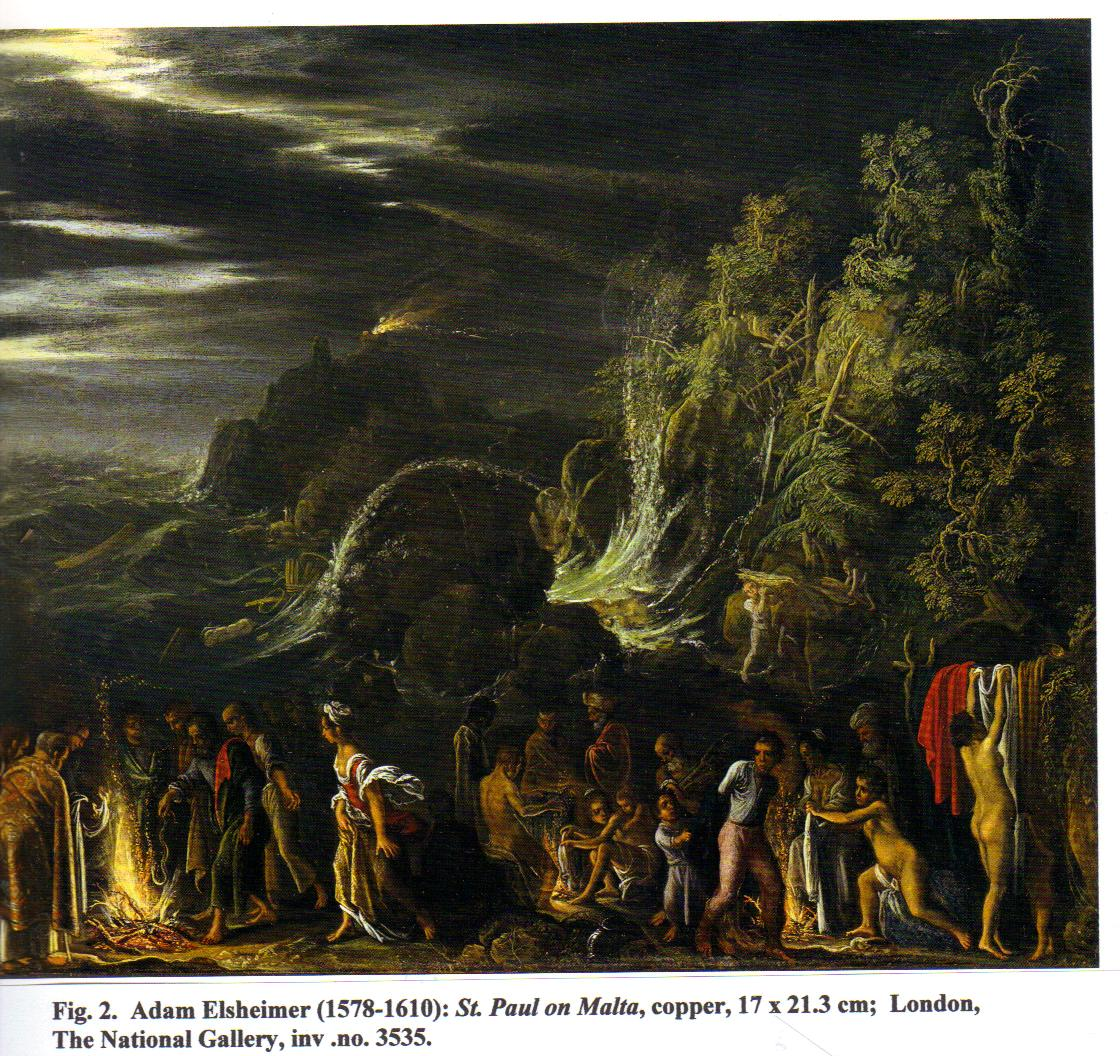
\includegraphics[width=10cm]{fig2.jpg}
%\caption{\it Adam Elsheimer (1578-1610): St. Paul on Malta,
%  copper, 17 x 21.3 cm;  London, The National Gallery, inv .no. 3535.}  
\end{figure}
First and foremost, by choosing a night scene
Elsheimer was free to demonstrate features for which he became famous:
an extraordinary range of the effects of light, particularly as it
illuminated the natural world.  Thus our eyes are immediately drawn to
the drama of a horrendous storm.  It occupies the upper two-thirds of
the panel: an area of general darkness, where diagonal beams of light
from sky and from a lighthouse give brief glimpses of rocky coast,
leaping spray, wreckage and fallen trees.  One tiny figure can just be
seen emerging from the debris.

Impressive as this is as a shipwreck, Elsheimer's personal
understanding of the landing of St.~Paul only becomes clear within the
lower third of the panel, where a horizontal strip of stony ground
extends along its lower edge, creating an area that is visually all
but separated from the turmoil above.  It is packed with figures, in
this case discernible to a greater or lesser degree by the light of a
fire near the left margin.  Within a group around this fire, light
catches the outline of a snake and the red mantle of a bare-footed
St.~Paul, a figure otherwise differing little from those leaning
forward to watch him in quiet wonderment.  Along the remainder of this
lower edge all is quiet activity: the removal and drying of their
clothes by a group of men, women and children in various stages of
undress.  There are no social distinctions here, and some are helping
others as they struggle to pull off their soaked garments and hang
them up to dry.  For this artist then, the fact of being saved by
Divine Providence has not only rendered the passengers outwardly
indistinguishable one from another, but with the recognition of a new
reality, each individual exhibits a quiet readiness and helpfulness -
an atmosphere that brings into line the figure glimpsed in the upper
section, leaving the devastation with a confident step, to join his
companions with his contribution of firewood.  Moreover, their
salvation has come from a saint seen both as unassuming and untiring,
who, having reached the shore, continues his mission.

It is the untiring strength of purpose of St.~Paul that is depicted
metaphorically by a present-day artist, Clive Uptton, who shows the
saint as a man of immense physical strength facing physical danger – a
rough sea.  Moreover, in his struggle to reach the coast he bears on
his shoulders a man to whom he is chained, and whose strength was
failing--the Roman centurion in whose charge he had been travelling to
Rome\footnote{For the centurion, Julius, see Acts 7.  Clive Uptton
  (1911--2006) was an artist whose wide range of illustrations
  included those for `The Story of Paul Retold', published in the
  magazine for children \textit{Look and Learn}, from which the one
  shown here, `The Great Shipwreck', is taken.}. [Fig.3]
\begin{figure}[htbp]
\centering
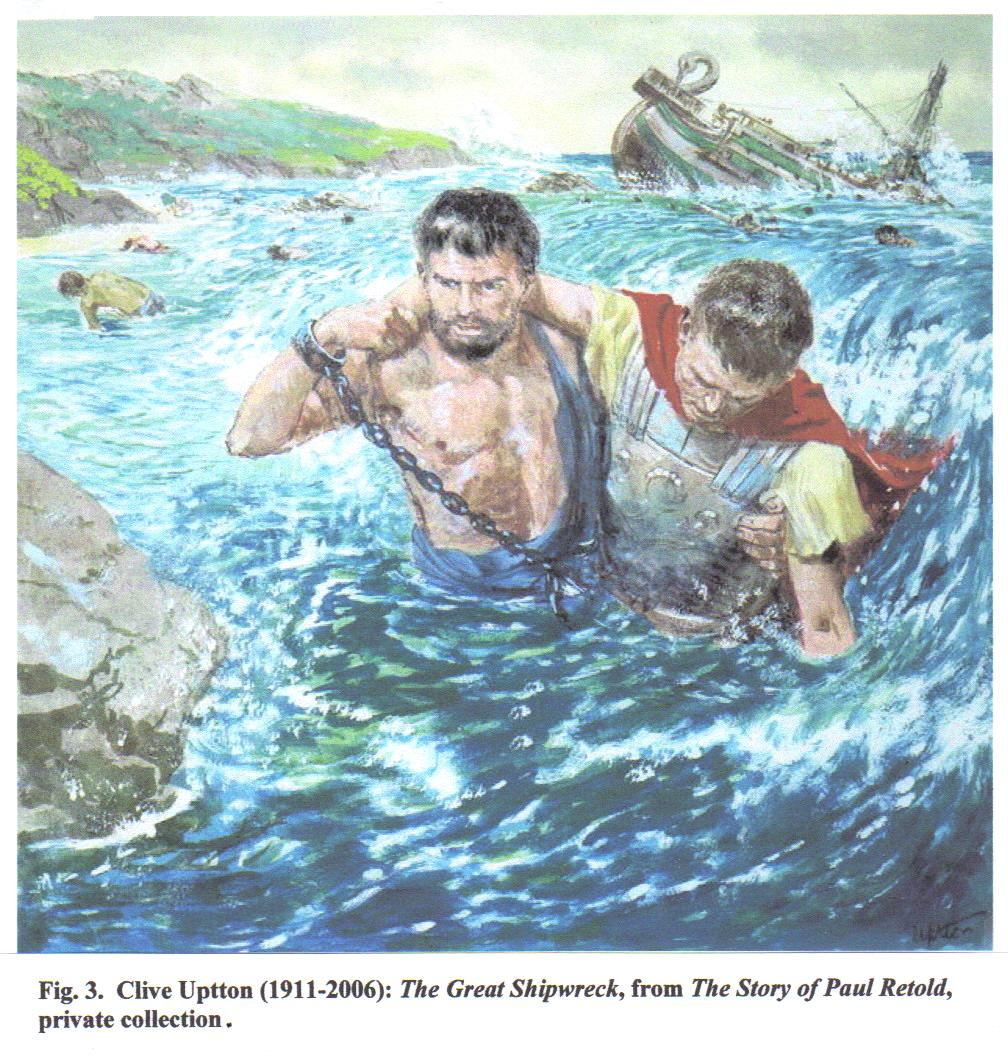
\includegraphics[width=8cm]{fig3.jpg}
\end{figure}

In these examples artists have focussed variously on the message
itself, the difficulties overcome and the courage of the messenger.
Thus with Eradi the nature of the message is powerful,
overwhelming--features he transposes to the commanding figure of the
messenger.  Elsheimer's main focus on the other hand is on the danger
that has been overcome in order to reach dry land – the terrifying
storm--and shows a saint who then quietly continues his mission,
whilst those who have followed him to safety have been granted the
blessings of a new life.  And Uptton visualises St.~Paul's untiring
strength of purpose, in terms of physical strength at a time of
physical danger--a strength he employs in the rescue of one in dire
need of assistance.


Placed side by side, the individually different visions of
artists celebrating a momentous event are found to be complementary,
and taken together they cannot but deepen our understanding of the
subject.

\end{document}
